%*********************************************************************
% gdutthesis: 广东工业大学论文模板
% 2021/11/09 v0.1c
%
% 重要提示:
%   1. 请确保使用 UTF-8 编码保存
%   2. 请使用 XeLaTeX 或 LuaLaTeX 编译
%   3. 请仔细阅读用户文档和 Wiki
%   4. 修改、使用、发布本文档请务必遵循 LaTeX Project Public License
%   5. 不需要的注释可以尽情删除
%*********************************************************************
\documentclass[
  % type=doctor
  type=master
  % type=promaster
]{gdutthesis}

% 宏包在这里加载
\usepackage{siunitx}[=v2]
\usepackage{zhlipsum,lipsum}

\gdutsetup{
  style = {
    cover           = {true},
    % cover           = {false},
    % font            = {garamond},
    % font            = {libertinus},
    % font            = {lm},
    % font            = {palatino},
    font            = {times},
    % font            = {times*},
    cjk-font        = {fandol},
    % cjk-font        = {founder},
    % cjk-font        = {mac},
    % cjk-font        = {sourcehan},
    % cjk-font        = {noto},
    % cjk-font        = {windows},
    % cjk-font        = {none},
    bib-backend     = {bibtex},
    % bib-backend     = {biblatex},
    bib-resource    = {gdutthesis-template.bib},
    bib-style       = {numerical},
    % bib-style       = {author-year},
    fullwidth-stop  = {mapping},
    % fullwidth-stop  = {catcode},
    % fullwidth-stop  = {false},
    hyperlink       = {color},
    % hyperlink       = {border},
    % hyperlink       = {none},
    hyperlink-color = {default},
    % hyperlink-color = {autumn},
    % hyperlink-color = {business},
    % hyperlink-color = {classic},
    % hyperlink-color = {elegant},
    % hyperlink-color = {fantasy},
    % hyperlink-color = {material},
    % hyperlink-color = {science},
    % hyperlink-color = {summer},
    % hyperlink-color = {graylevel},
    % hyperlink-color = {prl},
  },
  info = {
    title           = {模板射流电解加工微沟槽关键技术研究},
    title*          = {Investigation on masked jet electrochemical machining of micro grooves},
    date            = {2020/5/25},
    author          = {张三},
    author*         = {Zhang San},
    supervisor      = {李四\qquad 教授},
    supervisor*     = {Prof. Li Si},
    supervisor-two  = {王五\qquad 教授},
    supervisor-two* = {Prof. Wang Wu},
    department      = {自动化学院},
    department*     = {Automation},
    major           = {电子信息},
    student-id      = {2112101234},
    chairman        = {赵六\qquad 教授},
    degree          = {工程硕士},
    degree*         = {Master of Engineering},
    keywords        = {电解加工, 微沟槽, 模板, 射流},
    keywords*       = {electrochemical machining, micro grooves, mask, jet},
    secret-level    = {none},
  }
}


\begin{document}

\begin{abstract}
  \zhlipsum[1-4]
\end{abstract}

\begin{abstract*}
  \lipsum[1-4]
\end{abstract*}

\begin{notation}
  $E$ & 能量 \\
  $F$ & 推力
\end{notation}

\gduttableofcontents

\mainmatter

\gdutchapter{绪论}{Introduction}

\gdutsection{本课题研究背景及研究意义}{Background and significance of research}
随着科学技术的进步,产品逐渐向精密化和高性能化发展,具有毫米及微米尺度
微沟槽结构的金属零部件在国防军事、航空航天、新能源、新材料、生物医学、半导
体器件等领域的高技术产品中扮演的角色愈加重要。

\gdutsection{微沟槽电解加工国内外相关研究现状}{Analysis of the research status at home and abroad}
\gdutsubsection{成型电极电解加工}{Shaped cathode electrochemical machining}
采用与微沟槽结构形状对应的成型阴极,例如薄板阴极,片状阴极等,进行微沟
槽电解加工,其特点是方便一次成型微沟槽形状。南京航空航天大学吕焱明等进行了
大长宽比深窄槽电解加工阴极设计以及工艺试验研究\cite{chendengyuan2000guoshi},如\autoref{fig:example} 所示,具体参考\autoref{sub-fig-1} 和\autoref{sub-fig-2},再参考\autoref{eq:example},再再参考\autoref{tab:example}。
\begin{equation}\label{eq:example}
  E = mc^2
\end{equation}

\begin{figure}[htbp]
  \subfloat[贴有模板的金属喷嘴示意图]{\label{sub-fig-1}
    \includegraphics[width=0.4\textwidth]{example-image.pdf}
  }
  \qquad
  \subfloat[由点到线扫描加工原理图]{\label{sub-fig-2}
    \includegraphics[width=0.4\textwidth]{example-image.pdf}
  }
  \bicaption{模板射流电解加工微沟槽原理图}{Principle of masked jet electrochemical machining of micro grooves}
  \label{fig:example}
\end{figure}

\begin{table}
  \bicaption{DMC5400A 运动控制卡主要技术指标}{DMC5400A main specifications}
  \label{tab:example}
  \begin{tabular}{cc}
    \toprule
    控制卡技术指标              & 具体参数                      \\
    \midrule
    控制电机的脉冲信号频率范围  & $\SI{1}{Hz}\sim\SI{2}{MHz}$ \\
    控制电机的脉冲信号频率精度  & \SI{0.0625}{Hz}              \\
    脉冲信号输出最大电流        & \SI{20}{mA}                  \\
    脉冲信号长度                & 28 位有符号                   \\
    直线插补精度                & $\pm \SI{0.8}{pulse}$        \\
    圆弧插补精度                & $\pm \SI{1.5}{pulse}$        \\
    支持的插补坐标系个数        & 2                             \\
    \bottomrule
  \end{tabular}
\end{table}


\subsubsection{微沟槽电解加工国内外相关研究现状}
测试 test。
\paragraph{测试 test。}
测试 test。
\subparagraph{测试 test。}
测试 test\cite{woerdelun2012jingji}。

\gdutchapter{传感器融合}{Sensor fusion}
本章介绍了我们开发的一种适用于多旋翼飞行器的传感器融合算法,使用IMU作为主要传感器。我们感兴趣的是在飞行器平台上运行的状态估计算法,这种应用场景对于传感器融合有不一样的要求。因此,我们针对这些系统需求处理传感器融合、异常处理等问题。\par
我们注意到,这个课题已经有很好的研究成果\cite{mahony2008nonlinear,hua2010attitude,khosravian2016state}。我们的工作与现有成果之间的主要区别在于,我们的系统整合了现有成果的方法,具有很强的鲁棒性。我们确保该系统能够在大震动、高机动环境中稳健运行,在这些环境中,依赖单一现有成果的算法是不可行的。我们给出了高机动运行环境下的实验结果,要求系统在一段较长的时间内无故障运行。\par

\begin{figure}[htbp]
	\centering
	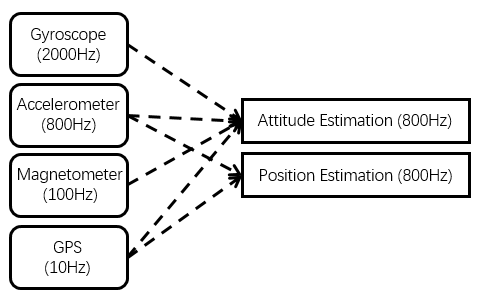
\includegraphics[width=0.7\textwidth]{state estimation.png}
	\bicaption{状态估计框架图}{Diagram of state estimation}
	\label{fig:stateestimation}
\end{figure} 

在本章中,我们将重点讨论系统中使用的状态估计方法(\autoref{fig:stateestimation})。我们将介绍由这些方法支持的系统飞行测试结果。我们注意到,自主飞行需要仔细地集成其他重要模块,如规划、控制和地面站。然而,我们希望将这些模块的集成的讨论放到到第五章,因为它们中的大部分都是对其特定领域中现有结果的直接应用。这些模块作为通用模块,以支持整个系统的运行。

\gdutsection{姿态估计}{Attitude estimation}
我们工作的核心是一个可靠的估计模块,该模块使用GPS和低成本的IMU输出姿态。我们注意到,基于磁力计及GPS的偏航角估计较为特殊,因此,基于低成本传感器的特性,我们提出了一种解耦估计器设计。\par
我们将世界坐标系和机体坐标系中的向量分别定义为$(\cdot)^w$和$(\cdot)^b$。我们感兴趣的是世界坐标系中飞行器的姿态,其定义为$\begin{bmatrix}
	\phi^w & \theta^w & \psi^w
\end{bmatrix}$。其中$\psi^w$、$\theta^w$和$\phi^w$是偏航角、俯仰角和横滚角,表示经过ZYX欧拉角转换后从机体坐标系到世界坐标系的旋转。因此,我们有旋转矩阵表示
\begin{equation}\label{eq:rotationmatrix}
	R_{b}^{w}=R(\psi^w)R(\theta^w)R(\phi^w)
\end{equation}\par
我们使用基于多传感器融合的姿态估计方法来估计三维姿态。一种带延时观测的显式互补滤波器(ECF)将IMU数据与GPS融合,以提供横滚角($\phi^w$)和俯仰角($\theta^w$)的估计。解耦估计器将陀螺仪数据、磁力计数据和GPS融合,以提供偏航角($\psi^w$)的估计。

\gdutsubsection{横滚角、俯仰角估计}{Roll and pitch estimation}
直接安装在机体的IMU作为横滚角和俯仰角估计的主要信息来源。我们评估了几种基于IMU的姿态估计方法,如基于非线性观测器的方法\cite{mahony2008nonlinear}、基于扩展随机线性估计的方法\cite{sabatelli2012double}和基于粒子滤波的方法\cite{cheng2004particle}。然而,由于飞行器的机动性需要以200Hz以上的更新速率进行姿态估计,而我们有限的板载计算资源,因此我们选择了基于非线性观测器的算法,该算法可以产生鲁棒且低算力的实时姿态估计。我们利用GPS的速度观测\cite{hua2010attitude}来处理飞行器运动状态下的姿态估计问题。 

\gdutsubsection{偏航角估计}{Yaw estimation}
我们以四元数为状态的CF融合陀螺仪、磁力计和GPS进行偏航角估计。我们通过观测指向磁北的向量以及GPS速度都能得出世界坐标系的偏航角误差。如果磁力计得出的偏航角误差变化太大,通常是由于飞行器外部磁场变化导致的,我们放弃当前的磁力计测量数据,并推迟测量更新,直到获得稳定的测量。在磁场干扰环境下,考虑使用GPS速度数据进行融合。如果没有稳定的偏航角测量值可用,这些测量值增强了系统的鲁棒性。当磁力计数据不可用时,我们使用GPS速度进行短期测量更新,迫使飞行器在小范围进行运动。\par
后面的小节中将介绍一种更有原则性的方法,将GPS测量值和磁力计测量结合起来,总体提供偏航估计。通过融合两种信息来解决磁场干扰引起的偏航误差修正问题。

\gdutsection{基于ECF的传感器融合}{ECF-based sensor fusion}
本节介绍了$SO(3)$上非线性互补滤波的一般框架。为了确保输出能满足反馈控制的高频、准确和无漂移的姿态估计,我们使用显式互补滤波器(ECF)融合并将姿态估计频率提高到800Hz。ECF结合10Hz的GPS数据、100Hz的磁力计数据、2000Hz的陀螺仪数据和800Hz的加速度数据,提供800Hz的姿态估计估计(\autoref{fig:stateestimation})。最终的估计输出平均延迟为0.01s,直接反馈到飞行器的反馈控制回路进行姿态控制。
\par
姿态估计的目标是为估计量$\hat{R}(t)\in SO(3)$提供一组动力学方程来使得误差旋转矩阵$\widetilde{R}(t)\rightarrow I_3$。真实系统的运动学方程为
\begin{equation}\label{eq:kinematics}
	\dot{R}=R\Omega_{\times}=(R\Omega)_{\times}R
\end{equation}\par

本文的ECF的状态向量定义为
\begin{equation}\label{eq:statevector}
	x_{t}=
\begin{bmatrix}
	q_{b}^{w} & b
\end{bmatrix}^T
\end{equation}
其中,$q_{b}^{w}=\begin{bmatrix}
	q_w & q_x & q_y & q_z
\end{bmatrix}^T$是$t$时刻的姿态四元数,,$b=\begin{bmatrix}
 b_x & b_y & b_z
\end{bmatrix}^T$是$t$时刻的陀螺仪零偏。注意,$q_{b}^{w}$表示的是$t$时刻机体坐标系相对于世界坐标系的姿态。$b$表示的是机体坐标系下的陀螺仪零偏。考虑\autoref{eq:kinematics}的旋转运动学方程,则对应的四元数运动学方程为
\begin{equation}\label{eq:quatkinematics}
	\dot{q}=\frac{1}{2}q\otimes \mathbf{p}(\Omega)
\end{equation}\par
基于IMU的姿态估计首先将加速度计测量值转换为世界坐标系,然后用于测量更新。测量值模型可以写成
\begin{equation}\label{eq:measurementmodel}
	a=R^T(\dot{v}-g)+b_a+\mu_a
\end{equation}
其中$v$表示机体系相对于世界系的瞬时线性加速度,$\mu_a$为测量噪声。由于姿态测量模型是非线性的,不可以通过卡尔曼更新步骤进行测量更新。因此我们采用非线性滤波器的思路进行设计。\par
本文使用的ECF后来发展成为基于ECF的多传感器融合框架,以一致的方式将来自磁力计和GPS的信息进行组合。

\gdutsection{位置速度估计}{Position and velocity esitimation}
我们通过三阶互补滤波算法来解决位置速度估计问题。基于GPS和IMU,我们通过三阶互补滤波算法来修正位置速度误差。位置速度估计算法运行频率为800Hz。为了修正传感器延时引起的修正不一致,我们采用基于延时的算法\cite{khosravian2016state}。\par
注意,如\autoref{fig:stateestimation}所示,位置速度估计模块和姿态估计模块运行在同一个的进程中,运行频率一样。这样,姿态、速度和位置的延迟能统一对齐。

\gdutsubsection{考虑延时的三阶互补滤波}{Third order complementary filter with sensor delay}
根据IMU和GPS的数据,我们可以生成平滑准确的三维位置速度,用于飞行器控制。

\gdutsection{实验结果}{Experimental results}
本章给出了两个实验:(1)与信号良好的GPS/RTK的位置、速度及差分的加速度比较,研究了估计器的性能;(2)飞行器的飞行实验;第1章讨论了实验平台的结构。第四章将介绍控制方法。

\gdutsubsection{评估估计器的性能}{Evaluating estimator performance}
我们希望通过与真值对比以研究估计器的性能,真值是由厘米级精确度的GPS/RTK系统定义的。本小节的实验分为两部分。第一部分为飞行器飞行时,通过比较板载估计器输出与的GPS/RTK来评估估计的准确性。在本次实验中,估计器能很好地跟上GPS/RTK输出的真值。第二部分考察了使用来自估计器的姿态和速度反馈来维持姿态、速度和位置的反馈控制。

\gdutsubsection{飞行器飞行实验}{UAV flying test}

\gdutsection{总结与讨论}{Summary and discussion}
在本章中,我们展示了使用IMU作为主要传感器,融合其他传感器进行状态估计以实现飞行器的稳定飞行。关键技术是考虑了传感器延时,运动加速度补偿以及异常处理相关的算法。此外,我们将容易受到磁场干扰的偏航角和俯仰、横滚角解耦以保证系统的鲁棒性。本文提出的算法可以使飞行器保持稳定。

\gdutchapter{传感器校准}{Sensor calibration}
在本章中,我们研究如何使用较少的仪器来进行高精度的传感器校准以提供更好的传感器数据。一般来说,基于MEMS的传感器的精度都比较差,远远达不到高精度导航的要求。然而,开发基于MEMS的传感器的飞行器,要保证传感器数据精度是很困难的。在本章中,我们研究传感器校准算法,开发了一种不需要外部设备就可以进行较高精度的校准。我们详细介绍了基于优化的传感器校准算法,并将其与融合和控制方法(第4章)结合起来进行实验,以验证系统的性能。\par
本系统的关键技术是一种传感器校准算法,能够无需外部设备的情况下进行校准。我们要求校准算法能够使用人手就能完成,无需外部设备,在尽量简单的校准流程下保证校准结果的准确性。\par

\gdutsection{加速度计校准}{Acceleromter calibration}
首先建立加速度计的传感器模型,并利用重力的向量大小进行标定\cite{jekeli2012inertial}。对于加速度计,我们使用静态检测的方法\cite{fong2008methods},并使用基于方差的检测算法\cite{sabatini2006wavelet}。由于需要提取静止的重力向量,我们可以对原始数据进行静态检测,放宽校准种严格的静止的条件。利用校准后的参数将原始数据转化为标准的重力向量$g$。\par
我们的检测器基于基于Tedaldi的方法:对于每个加速度计样本$\begin{bmatrix}
	a^t_x & a^t_y & a^t_z
\end{bmatrix}$,给定一个长度为t秒的时间间隔时刻,我们计算方差的大小
\begin{equation}\label{eq:var}
	\zeta(t)=\sqrt{[var_{t_w}(a^t_x)]^2+[var_{t_w}(a^t_y)]^2+[var_{t_w}(a^t_z)]^2}
\end{equation}
其中$var_{t_w}(a^t)$是一个运算符,计算加速度计$a^t$在以$t$为中心,长度为$t_w$秒的时间间隔内的方差。我们通过判断$\zeta(t)$是否小于或大于一个阈值对静态和运动间隔进行分割。与传统的六面校准法相比\cite{尹杭2014一种},该方法在可以在任意姿态下保持静止。

\gdutsubsection{传感器误差模型}{Sensor error model}
对于加速度计,有
\begin{equation}\label{eq:axiserror}
	T^{a}=
	\begin{bmatrix}
		1 & \beta_{yz} & \beta_{zy}\\
		\beta_{xz} & 1 & \beta_{zx}\\
		\beta_{xy} & \beta_{yx} & 1
	\end{bmatrix}
\end{equation}
其中,$T^a$是轴正交矩阵,$\beta_{ij}$是第$i$个传感器轴的误差对第$j$个轴的造成的误差影响。\par
此外,加速度计受到零偏和尺度误差的影响。引入尺度矩阵
\begin{equation}\label{eq:scaleerror}
	K^{a}=
	\begin{bmatrix}
		s^a_x & 0 & 0\\
		0 & s^a_y & 0\\
		0 & 0 & s^a_z
	\end{bmatrix}
\end{equation}
我们接着引入零偏向量
\begin{equation}\label{eq:scaleerror}
	b^{a}=
	\begin{bmatrix}
		b^a_x\\
		b^a_y\\
		b^a_z
	\end{bmatrix}
\end{equation}
完整的传感器误差模型为
\begin{equation}\label{eq:sensorerrormodel}
	a^O=T^a K^a (a^S + b^a + \nu^a)
\end{equation}
其中,$a^O$和$a^S$分别表示校准后和校准前的加速度数据,$ν^a$是加速度计测量噪声。

\gdutsection{陀螺仪校准}{Gyroscope calibration}
一般来说,对于陀螺仪校准,要完整校准出零偏、尺度和轴正交要比加速度计校准复杂得多。即使对角速度精度有较高得要求,由于缺乏相应的设备,也无法校准出陀螺仪的尺度和轴正交参数。简单的陀螺校准无法用于高精度的导航上。因此,基于Tedaldi的方法\cite{tedaldi2014robust},我们将对陀螺仪进行十二参数的标定。

\gdutsection{磁力计校准}{Magnetometer calibration}
磁力计本身的系统误差非常大,直接用原始数据计算偏航角的精度十分差以至于无法用于控制飞行器的偏航。因此,我们基于椭球拟合的方法来校准磁力计\cite{李勇2012基于椭球拟合的三轴磁传感器误差补偿方法}。我们使用牛顿迭代法求解最小二乘问题,因为代价函数是非线性的。传感器测量模型与章节3.1相同。

\gdutsection{实验结果}{Experimental results}
实验环境不需要任何外部设备。在所有的实验中,我们只需要采集传感器的原始数据。实验平台在第1章中进行了讨论。实验平台是基于开源飞控。这个现成的飞控板配有一个IMU、一个磁力计和一个STM32微控制器。

\gdutsubsection{加速度计校准结果}{Accelrometer calibration result}
在本实验中,采集IMU原始数据,使其以任意姿态静止。整个校准流程为3分钟。校准精度是根据重力模长进行评估的。加速度计校准结果显示在。

\gdutsubsection{陀螺仪校准结果}{Gyroscope calibration result}
这个实验给出陀螺校准结果。陀螺仪和加速度计同时校准。校准精度是根据角度误差来评估的。陀螺仪校准结果显示在。

\gdutsubsection{磁力计校准结果}{Magnetometer calibration result}
在本实验中,采集磁力计原始数据,以足够多的姿态运动飞控。校准精度根据磁场模长进行评估。磁力计校准结果显示在。

\gdutsection{总结与讨论}{Summary and discussion}
在本章中,我们提出了一种IMU校准算法,该方法能够在无需外部设备的情况下进行校准。我们对校准评估标准方法的进行优化。我们的方法能够使精度提高到xxx。

\gdutchapter{控制}{Control methods}
本章讨论如何调整控制方法,以配合飞行器稳定飞行的需要。我们介绍了保证状态估计和控制平滑的系统体系结构。

\gdutsection{反馈控制}{Feedback control}
在给定估计的状态后,我们让飞行器用位置跟踪控制器来跟踪所需的轨迹\cite{lee2010geometric}。由传感器融合模块(第二章)的状态估计直接作为控制器的反馈。在本文的设计中,姿态控制器和位置控制器都在STM32以400Hz的频率运行。

\gdutsection{实验结果}{Experimental results}
我们有一个基于多传感器融合的状态估计器来产生800Hz的位置、速度、姿态估计,足以稳定飞行器。\par
在这个实验中,飞行器以大约1米/秒的速度自动沿着矩形轨迹生成平滑轨迹。使用GPS/RTK在信号良好的状态下来量化全局跟踪性能。由图xxx可以看出,飞行器的实际位置收敛到期望位置,其标准差为xxx,表明控制器的稳定收敛。

\gdutbackmatter
\gdutchapter{结论与展望}{Conclusion and prospect}
在这篇论文中,我们展示了对飞行器自主飞行的最新技术的贡献,大部分贡献是状态估计算法。在第三章中,我们开发了状态估计系统,提出了一种模块化和可扩展的方法,该方法能够以一致的方式组合来自多个传感器的信息。在第四章中,我们开发了传感器校准算法,能够在没有外部设备的情况下对传感器进行高精度的校准。在第五章中,我们提出的控制方法结合前两章的算法形成一个集成的飞行器系统。\par
我们注意到,虽然主要的实验平台使用的是四旋翼,但我们的方法不限于这一特定类型的平台。实际上,我们的方法是基于传感器的,同样适用于其他机器人,如固定翼、地面机器人等。
\gdutbacksection{成果总结}
综上所述,本文的主要贡献如下:
\begin{itemize}
	\item 我们开发了算法和系统,使计算资源受限的飞行器能够自主飞行,只使用低成本的传感器。
	\item 我们提出了一种算法,通过互补融合来自多传感器的信息来提高系统的可靠性。
	\item 我们提出了一种算法,无需外部设备就能够进行传感器校准。
	\item 我们开发集成了控制算法,并通过大量的实验表明,飞行控制系统是稳定可靠的。
\end{itemize}

\gdutbacksection{未来研究展望}
本文涉及到了几个有趣的研究领域,其中一些是随着飞行器技术的发展而不断发展成大型系统的,而另一些则是我们在评估最新方法的性能时值得追求的新方向。
\paragraph{自主飞行中估计与控制的耦合设计。}
在我们目前的工作中,控制器与估计器是分开设计的。然而,随着我们朝着高速自主飞行的方向发展,我们可能会要求估计器和控制器耦合设计,以生成和执行高效、无碰撞和安全的飞行轨迹。
\paragraph{用于飞行器的新的传感器技术。}
虽然传统的传感器如IMU、GPS、相机已被证明可用于飞行器导航,但最近传感技术的发展可能创造新的机会。例如,光场可以作为深度感知的传感器。这些新型传感技术在飞行器上的应用具有很大的潜力。
\paragraph{传感器和能观性研究。}
众所周知,传感器数量越多,系统的能观性越好,但单个传感器对系统能观性的影响尚不清楚。增加更多的传感器会带来出更多的能观性,但是传感器提供的信息以及信息的质量会导致能观性的复杂判断条件。因此,一个能够以在线方式识别能观性的通用框架将有利于更高层次的任务,如运动规划和风险评估。

\nocite{*}% 列出全部参考文献
\printbibliography

\gdutchapter{攻读学位期间取得与学位论文相关的成果}{Publication and patents during study}

\gdutbacksection{发表和投稿与学位论文相关学术论文}

\begin{results}
  \item \textbf{张三}, 李四, 等. Jet electrochemical machining of micro dimples with conductive mask.
  Journal of Materials Processing Technology. 2018, 257:101-111. (SCI Impact Factor 3.647,
  WOS:000431161400010)
  \item 李四, \textbf{张三}, 王五, 等. Electrochemical direct-writing machining of micro- channel array.
  Journal of Materials Processing Technology. 2019, 265:138-149. (SCI Impact Factor 3.647,
  WOS:000451935100014)
\end{results}

\gdutbacksection{申请发明专利}

\begin{results}
  \item 李四, \textbf{张三}, 王五. 一种微流道电解加工装置. 发明专利申请号: 201810467763.5.
\end{results}

\gdutstatement

\gdutchapter{致谢}{Acknowlegements}
\zhlipsum[1]

\gdutappendix

\gdutchapter{附录标题}{The appendix title}
对需要收录于学位论文中且又不适合书写于正文中的附加数据、资料、详细
公式推导、计算机程序等有特色的内容,可做为附录排写。
\end{document}